\chapter{The Design and Development of the Immotion Exergame}\label{chapter:implementation}

This chapter outlines the design and development of the Immotion exergame for warm up routine guidance and motivation. We begin with the description of the design methodology used for the development. For the purpose of this thesis, an iterative and prototype driven, user centered design has been adopted. Next, we cover the main development iterations
that have been undertaken during the exergame development process. 

\subsection{Overview of User Centered Design}

\subsection{Overview of the Development Phases}
The development of the Immotion exergame consisted of three primary phases which are according to the well accepted game design phases outlined by Furher and are depicted in Figure \ref{fig:iterations}: 
\begin{itemize}
\item Requirements gathering 
\item First prototype development with user evaluation
\item Final exergame development with further user evaluation
\end{itemize}
In the following sections, each iteration presented in Development section of Figure \ref{fig:iterations} will be further detailed. 
\begin{figure}[h]
    \centering
    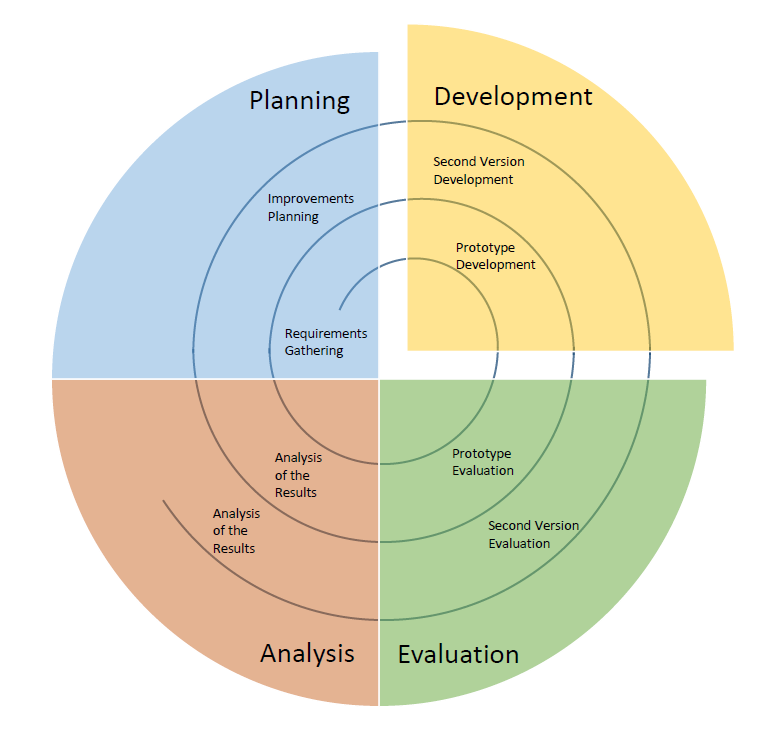
\includegraphics[width=\textwidth]{iterations}
    \caption{Overview of the development iterations}
    \label{fig:iterations}
\end{figure}
\section{Requirements Gathering}
This iteration was an exploratory step that justified the development and identified the currently available solution in the domain of exergames for warm up before sports activities. This was achieved through initial literature review which identified the most important areas to be addressed when developing gamified solution in the given context. TODO. Discussions with TAs?
\section{Prototype Development}
This section outlines the development of the prototype version of the exergame for warm up before sports activities. Our primary goal with the prototype was to develop a working version of the game that can process movements in real time in order to guide users through the warm up routine and, presumably immerses the participants sufficiently so that their focus is shifted from the discomfort and exertion of the exercise towards the enjoyment of the experience.

\subsection{Game Description}
The Immotion exergame has been created using the Unity 5.6 game development platform developed by Unity Technologies []. User's movements were captured and processed using Kinect for Xbox One (2.0 2013) motion sensing input devices by Microsoft []. The game engine was run on XX [] and projected on a wall using XX projector. In figure \ref{fig:hs} we outline the relationship of the game, software, and hardware equipment.
\begin{figure}[h]
    \centering
    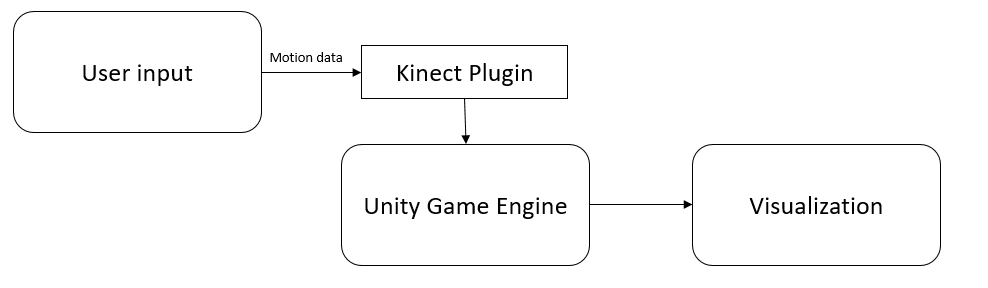
\includegraphics[width=\textwidth]{hardware_software}
    \caption{Hardware and Software supporting the prototype exergame}
    \label{fig:hs}
\end{figure}\\
For the prototype version of the exergame, a game scenario that is similar to Subway Surfers [] and Temple Run [] games has been implemented. In these games, the player controls the character that is on a track and needs to move left, right or jump up in order to avoid obstacles and collect points. In our solution, the player controls the character by doing a set of movements, which are tracked using a Microsoft Kinect device. In-game obstacles and coins were position in a way that the user was required to perform a specific movement. By avoiding obstacles and collecting coins the overall user score was increased. Our intention was to indirectly promote exercise through the gameplay of repeatedly performing warm up related movements by avoiding obstacles and collecting coins.

\subsection{Gamification Elements}
Werbach and Hunter [] (2012) report that \textit{Mechanics} provide the ''basic processes that drive the action forward and generate
player engagement''. For the prototype version of the Immotion exergame, the most important mechanics was \textit{Feedback}.

\subsubsection{Feedback}
As pointed out in Chapter \ref{chapter:relatedwork}, feedback have been shown to influence and improve autonomy and, hence, the intrinsic motivation of individuals [Ryan 2006]. Warbach and Hunter argue that giving unanticipated, informal feedback or support about the player's progress can provoke increased intrinsic motivation and autonomy []. In the context of the prototype version of the Immotion exergame, the feedback has been given by the amount of points acquired by collecting the coins during the gameplay.
\subsection{Points}
According to Zichermann and Cunningham [] (2011) points are ``an absolute requirement for all gamified systems'' since they can serve a wide range of purposes. One of the most obvious is for keeping a score and evaluate progress of the user. However, they can serve as a powerful extrinsic motivator for player types that enjoy collecting points, like \textit{Killers} or \textit{Achievers}. In the prototype version of the exergame, user could earn points only by collecting coins and lose them by hitting an obstacle. How much points could the player earn or lose by each action is presented in Figure \ref{fig:points}.
\begin{figure}[h]
    \centering
    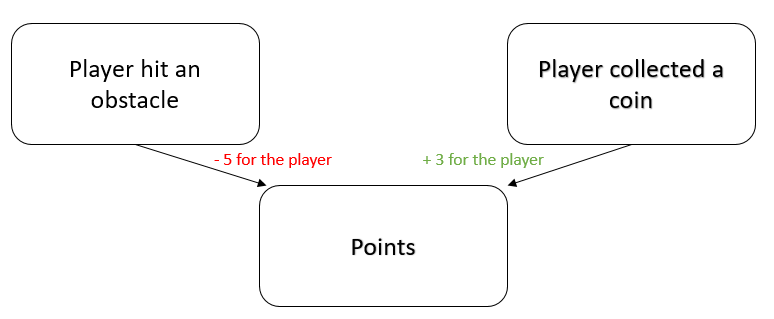
\includegraphics[width=\textwidth]{points}
    \caption{Earning and loosing point in the prototype version of the exergame}
    \label{fig:points}
\end{figure}\\
As per Figure \ref{fig:points}, the player could earn 3 points by collecting a coin. Contrarily, the player could lose 5 points if hit by an obstacle. In order to avoid hitting an obstacle or collect a coin, a movement was required to be performed by the player. Consequentially, the player was guided through the warm up routine without even realizing it.
\begin{figure}[h]
    \centering
    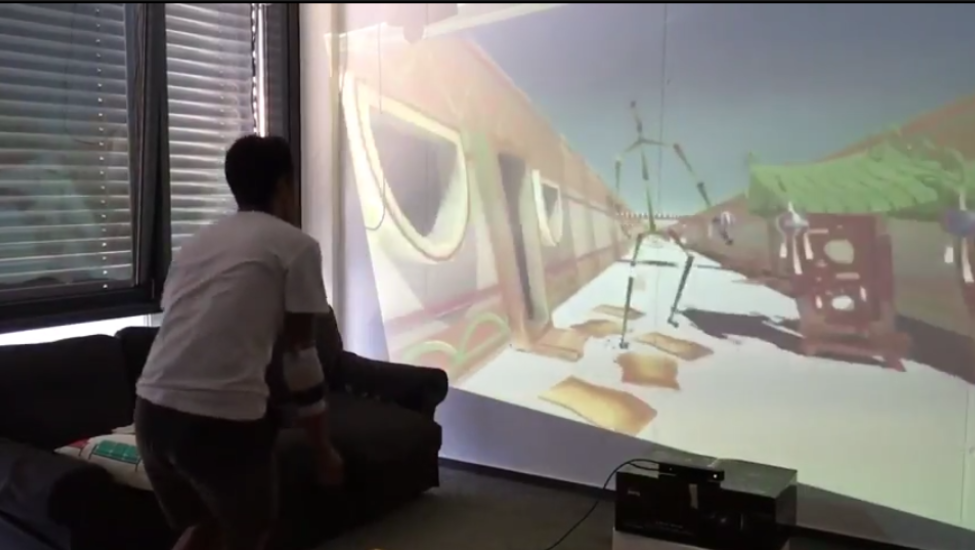
\includegraphics[width=\textwidth]{proto0}
    \caption{Earning and loosing point in the prototype version of the exergame}
    \label{fig:prototype_usage}
\end{figure}
\begin{figure}[h]
    \centering
    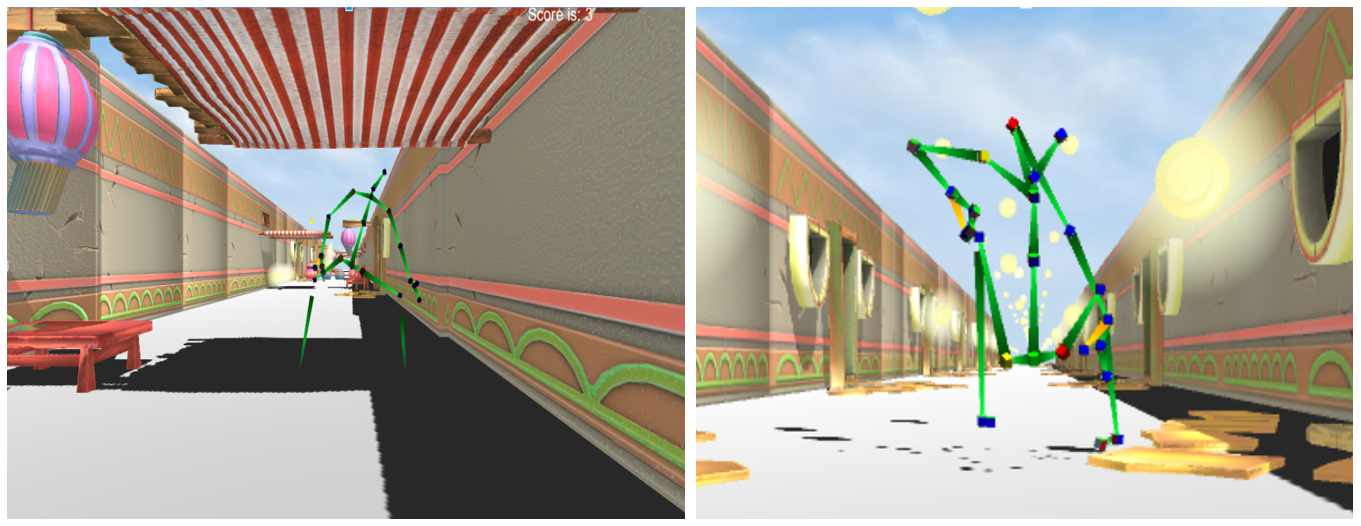
\includegraphics[width=\textwidth]{prototype}
    \caption{Earning and loosing point in the prototype version of the exergame}
    \label{fig:prototype}
\end{figure}
\subsection{Game Scenes}
\section{Final Exergame Solution}